% 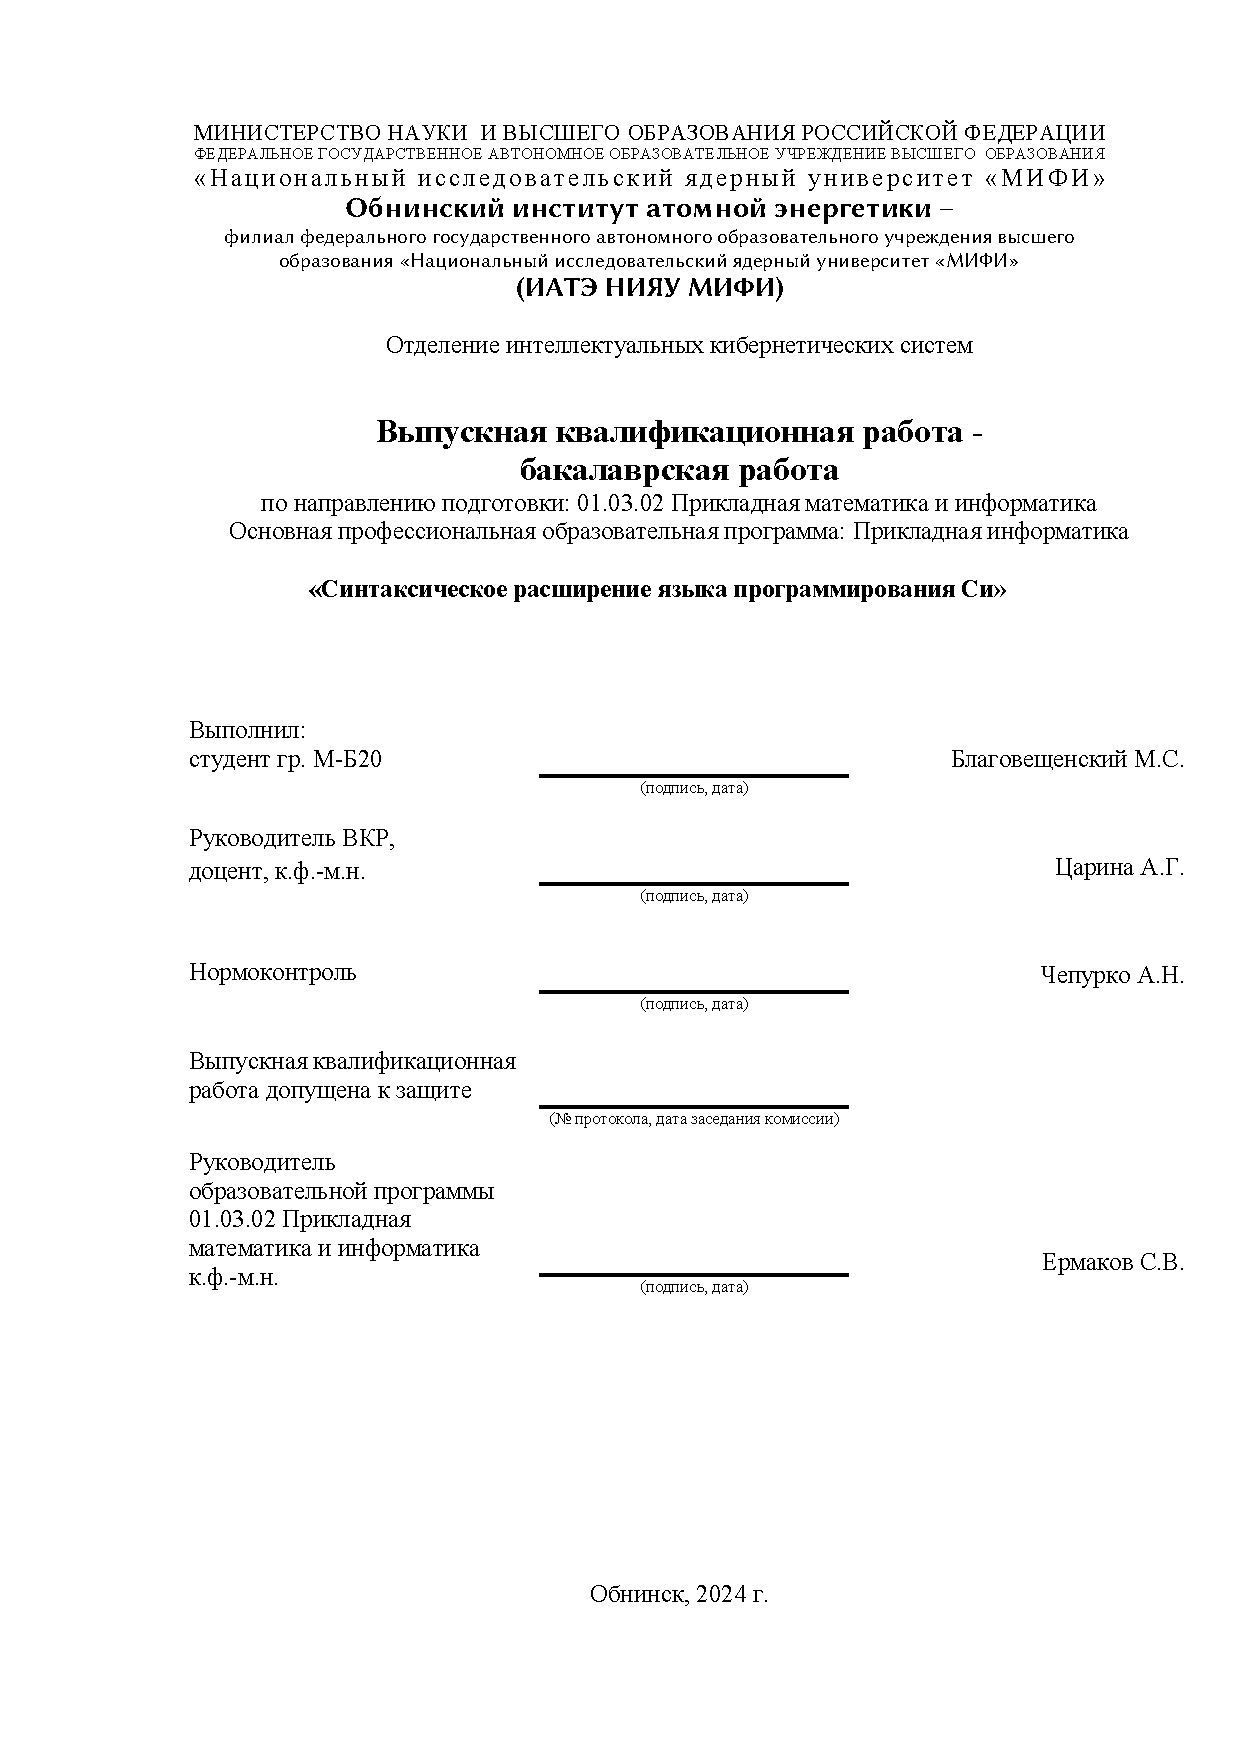
\includepdf[pages={-}]{title_page}

% \section*{Постановка задачи}
% Изучить стандарт\cite{c23_std} языка Си.
% Написать лексический анализатор языка Си. 
% Написать библиотеку грамматического разбора языка Си. 
% Рассмотреть приложения использования данной библиотеки в контексте метапрограммирования.
% \addcontentsline{toc}{section}{Постановка задачи}


\newpage
\section{Определения}

\begin{enumerate}
\item Лексема(Токен) - элементарная единица языка с точки зрения его грамматики. Может состоять из нескольких символов.
Примеры: ',' - запятая, '...' - троеточие, 'имя' - идентификатор, '"text"' - строковой литерал

\item CFG - Context-Free Grammar (контекстно-свободная грамматика)

\item AST(АСД) - Abstract Syntax Tree (абстрактное синтаксическое дерево)

\item Дерево - связный граф, у каждого элемента которого не более одного предка

\item Аллокатор - абстракный объект, предоставляющий интефейс выделения/возврата памяти из кучи(heap)

\item Стек(Stack) -  структура данных, представляющий собой список элементов, организованных по принципу LIFO (last in — first out, последним пришёл — первым вышел).
\end{enumerate}

\def\titlecite#1{\citetitle{#1}\cite{#1}}

\def\thminteddefaults{breaklines=true, xleftmargin=1em, linenos, frame=single, framesep=10pt, fontsize=\footnotesize}
\def\beginminteddef#1{\begin{minted}[
  breaklines=true, xleftmargin=1em, linenos, 
  frame=single, framesep=10pt, fontsize=\footnotesize]{#1}}

\newpage
\section{Введение}

\subsection{Актуальность проблемы}
Язык программирования - основной инструмент любого разработчика. 
На практике часто встречаются задачи, когда стандартных утилит для работы с языком недостаточно, и приходится писать свои собственные.
Цель данного проекта - помочь в разработке подобных утилит.

Разработчику предлагается использовать данную библиотеку для превращения программного кода в абстрактное синтаксическое дерево - 
структуру данных, которая может быть обработанно процедурно (программным путем).

% TODO
Си это язык со слабой статической типизацией.

\subsection{Постановка задачи}
Изучить стандарт\cite{c23_std} языка Си.
Расширить и протестировать существующий код библиотеки.
Написать препроцессор языка Си. 
Организовать интерфейс для данной библиотеки с помощью абстракции "Единицы трансляции" (Translation Unit)\cite{wiki-tr-unit}.

% \textbf{ecc} является source-to-source компилятором, т.е.компилятором, транслирующих текст программы на одном языке программирования в текст программы 
% на другом (возможно том же самом) языке программирования. 
% В данном случае после разбора текста синтаксическая надстройка на Си интерперетируется, после чего полученное в ходе интерпретации дерево компилируется к тексту языка Си.

Идея состоит в том, чтобы часть функционала компилятора Си, вынести в виде пользовательской библиотеки.
Необходимость такого функционала возникает, когда у разрабочка возникает потребность 

Си устоявшийся(stable) и стандатизированный язык, 
поэтому нет проблемы нестабильного API из-за постоянно развивающего языка, как например сейчас происходит в Rust.

\subsection{Обзор литературы}

\titlecite{c23_std}, \titlecite{c99_std} - основные документы, содержащие информацию о языке Си.

\titlecite{crafting_interpreters} - основная книга, использованная в данной работе. 
В ней продемострирован метод рекурсивного спуска, описан лексер и парсер для придуманного автором языка Lox.

\titlecite{hmu} - теория формальных языков, абстрактных вычислительных машин и грамматик. 
Данная книга использовалась как источник математического знания по теме на ранних этапах изучения.

\textit{The Theory of Parsing, Translation, and Compiling (Volume I, II)}
\cite{ptc_vI} \cite{ptc_vII} - классические книги по теории компиляции.

\titlecite{monparsing_paper}\titlecite{ml_syntax_transformation_paper} - статьи про монадические парсеры.

\titlecite{peg_paper} - оригинальная статья автора PEG грамматики.

\paragraph{Разбор выражений и приоритет операций}
% \caption{pratt}
\label{litover:pratt} \mbox{} \\
\titlecite{tdop_pratt_paper} - оргинальная статья автора \\
\titlecite{nystrom_pratt_parsers} - поясняющая статья с упором на практику \\
\titlecite{cppref_op_prec} - справка по языку Си: приоритет операций \\
\titlecite{pest_op_pratt} - парсер Пратта в фреймворке pest

\section{Обзор архитектуры проекта}

Требования к окружению:
OS: GNU/Linux
Наличие компилятора gcc

Проект выполнен как динамическая библиотека libecc.so %и небольшая утилита \verb|ecc| использующая ее.



\subsection{Сравнение с другими языками}
\subsubsection{Сравнение с языком C++}
Для C/C++ существует компилятор Clang, у которого frontend выненсен в качестве библиотеки, однако данный компилятор заточен больше на C++, что существенно услоожняет Ast, 
поэтому было принято решения написать свой минималистичный frontend для Си.

\subsubsection{Сравнение с языком Rust}
В Rust представленна система процедурных макросов, схожая с системой, выполенной в данной работе.

\subsubsection{Сравнение с языком Julia}


\subsubsection{Сравнение с языком Zig}
В языке Zig метапрограммирование выполненно с помощью функционала \verb|comptime| - позволяющего выполнять код во время компиляции и функционала рефлексии, 
позволяющего получить информацию о типе в виде \verb|comptime| структуры, что предоставляет гибкий интерфейс для расширения возможностей компилятора, не прибегая 
к сторонним утилитам.

\newpage
\section{Практическая часть: введение}

Разработана библиотека ec.so, в которой реализованны возможности source-to-source компилятора языка Си.
К этой библиотеке написана небольшая утилита \verb|ecc|, реализующая для нее cli интерфейс.
Данный функционал предоставлен пользователю для решения задачь метапрограммирования: предобработки, умной компиляции, и др.

Поверх стандартного фунционала разбора языка Си в библиотеку добавлено синтаксическое расширение языка: Extended C
Которое может быть использованно пользователем для разметки программного кода с целью последующей его обработки, что продемострированно далее 
% TODO add ref

Библиотека реализованна на языке C23, используется некоторые улучшения, добавленные в новом стандарте.

Используются:
\begin{enumerate}
  \item ключевое слово \textbf{auto} для автоматического вывода типов
  \item взятие адреса у литерала, например \verb|&(int) {3}|
  \item gcc выражения-утдверждения (statement expressions), вида \verb|({x = 3; x;})|
  \item gcc \verb|,##| оператор в макросах
\end{enumerate}


\subsection{Основные примитивы}
Для написания основной библиотки используюется дочерняя библиотека\ref{extras:c-core} с основными примитивами: 
строковыми, ввода-вывода, аллокации памяти и др.

Данная библиотека реализована в виде единичных самодостаточных заголовочных файлов, 
которые могут быть в зависимости от флага препроцессора либо заголовочными файлами либо файлами имплементации, 
по принципу stb библиотек\cite{stb_libs}.

\subsubsection{Макросы}

Для определений структур и энумераций используются следующие макросы:

\beginminteddef{c}
#define struct_decl(name) \
typedef struct name name; \
struct name; \

#define enum_decl(name) \
typedef enum name name; \
enum name; \

#define struct_def(name, fields) \
typedef struct name name; \
struct name fields; \

#define enum_def(name, ...) \
typedef enum name name; \
enum name {__VA_ARGS__}; \
\end{minted} 


\subsubsection{Обработка ошибок}

Ошибки кодируются как enum, например:

\begin{listing}
\caption{Ошибки Аллокатора}
\beginminteddef{c}
enum_def(AllocatorError,
    ALLOCATOR_ERROR_OK,
    ALLOCATOR_ERROR_MEM_ALLOC,
    ALLOCATOR_ERROR_COUNT
)
#define ALLOCATOR_ERROR(ERR) ((AllocatorError)ALLOCATOR_ERROR_##ERR)
\end{minted}
\end{listing}

Значение OK кодируется как 0, остальные значения кодируются положительными числами.

Для обработки ошибок используются следующие макросы:
% \begin{minted}[linenos, frame=single]{c}
\beginminteddef{c}
#define IS_OK(e) ({ \
    auto _r = (e); \
    *(int *)&(_r) == 0; \
    })
#define IS_ERR(e) ({ \
    auto _r = (e); \
    *(int *)&(_r) != 0; \
    })
#define TRY(expr) { \
    auto _e_ = (expr); \
    if (IS_ERR(_e_)) { \
        return _e_; \
    } \
  }
#define ASSERT(expr) \
    if (!(expr)) { \
        fprintf(stderr, "ASSERT at %s:%d:\n", __FILE__, __LINE__); \
        panic(); \
    } 
#define ASSERTM(expr, msg) { \
    if (!(expr)) { \
        fprintf(stderr, "ASSERTM: %*s\nat %s:%d:\n", (int)(sizeof(msg)-1), msg, __FILE__, __LINE__); \
        panic(); \
    } \
}
#define ASSERT_OK(expr) { \
    auto _e_ = (expr); \
    if (IS_ERR(_e_)) { \
        fprintf(stderr, "ASSERT_OK at %s:%d:\n", __FILE__, __LINE__); \
        panic(); \
    } \
}
\end{minted} 

\verb|IS_OK|, \verb|IS_ERR| - проверяют была ли ошибка

\verb|TRY| - если была ошибка верни ошибку из текущей функции 

\verb|ASSERT_OK| - если была ошибка, критическое завершение программы 

\subsubsection{Контекст}
Используется глобальный контекст, уникальный для каждого потока:

\beginminteddef{c}
__thread struct {
    Allocator global_alloc;

    Arena imm_str_arena;
    Allocator imm_str_alloc;
    slice_T(u8_t) dump_buffer;

    void (*raise)(Error);

    StreamWriter stdout_sw;
    StreamWriter stderr_sw;
} g_ctx;
\end{minted} 

\subsubsection{Аллокатор}
Используется интерфейс абстрактного аллокатора:

\beginminteddef{c}
AllocatorError
allocator_alloc(Allocator* self, usize_t size, usize_t alignment, void **out_ptr);
AllocatorError
allocator_resize(Allocator* self, usize_t size, usize_t alignment, void **in_out_ptr);
allocator_free(Allocator* self, void **ptr);

AllocatorError
allocator_alloc_z(Allocator* self, usize_t size, usize_t alignment, void **out_ptr);
\end{minted} 

Примерами такого аллокатора служат глобальный glibc аллокатор и арена алокатор 

\subsubsection{Арена Памяти}
Для оптимизации и удобства работы с памятью используется структура арены памяти.

\beginminteddef{c}
struct_def(ArenaChunk, {
    u8_t *cursor;
    usize_t data_size;
    u8_t data[];
})

struct_def(Arena, {
    list_T(ArenaChunk) chunks;
    usize_t default_chunk_data_size;
})
\end{minted} 


\subsubsection{Строки}
Строки и строковые "срезы" (позразумевается, что \textit{String} владеет паматью, т.к. хранит абстрактный аллокатор, 
 а \textit{str\_t} нет)

\beginminteddef{c}
struct_def(String, {
    uchar_t *ptr;
    usize_t byte_cap;
    usize_t byte_len; // in bytes
    Allocator allocator;
})

struct_def(str_t, {
    uchar_t *ptr;
    usize_t byte_len; // in bytes
})

typedef uint32_t rune_t;
\end{minted}

Подразумевается, что строки используют UTF-8 кодировку.

Тип \verb|rune_t| - unicode code point, число кодирующее символ в стандарте Юникод.

Интерфейс итераторов считывания/записи юникод символов:
\beginminteddef{c}
UTF8_Error
str_next_rune(str_t self, rune_t *out_rune, str_t *out_self);

/// @param[in, out] out_str should be preinit, len 4 guaranties success
UTF8_Error
str_encode_next_rune(str_t self, rune_t rune, str_t *out_self);
\end{minted}


\subsubsection{Потоки ввода вывода}

Интерфейс абстрактного потока вывода:

\beginminteddef{c}
enum_def(IOError, 
    IO_ERROR_OK,
    IO_ERROR_WRITE,
)
#define IO_ERROR(ERR) ((IOError)IO_ERROR_##ERR)

typedef IOError (StreamWriter_WriteFn)(void *, usize_t, uint8_t[]);
typedef IOError (StreamWriter_FlushFn)(void *);

struct_def(StreamWriter_VTable, {
    StreamWriter_WriteFn *write;
    StreamWriter_FlushFn *flush;
})
struct_def(StreamWriter, {
    StreamWriter_VTable _vtable;

    void *data;
})
\end{minted}

Тип \verb|OutputFileStream| - поток вывода в файл, реализующий привиденный ранее интерфейс.

\beginminteddef{c}
struct_def(OutputFileStream, {
    slice_T(u8_t) buffer;
    void *b_cursor;
    void *e_cursor;
    FILE *file;
})

AllocatorError
output_file_stream_new_in(FILE *ofile, usize_t buffer_size, Allocator alloc[non_null], OutputFileStream *out_self);
IOError
output_file_stream_write(OutputFileStream self[non_null], usize_t data_size, u8_t data[data_size]);
IOError
output_file_stream_flush(OutputFileStream self[non_null]);
StreamWriter
output_file_stream_stream_writer(OutputFileStream self[non_null]);
\end{minted}

Строки тоже реализуют этот интерфейс(приведено с имплементацией).

\beginminteddef{c}
IOError
output_string_stream_write(String self[non_null], usize_t data_size, u8_t data[data_size]);
IOError
output_string_stream_flush(String self[non_null]);
StreamWriter
string_stream_writer(String self[non_null]);

IOError
output_string_stream_write(String self[non_null], usize_t data_size, u8_t data[data_size]) {
    ASSERT_OK(string_reserve_cap(self, data_size));
    ASSERT_OK(string_append_str(self, (str_t) {.ptr = data, .byte_len = data_size}));
    return IO_ERROR(OK);
}
IOError
output_string_stream_flush(String self[non_null]) {
    return IO_ERROR(OK);
}
StreamWriter
string_stream_writer(String self[non_null]) {
    return (StreamWriter) {
        ._vtable = (StreamWriter_VTable) {
            .write = (StreamWriter_WriteFn *)output_string_stream_write,
            .flush = (StreamWriter_FlushFn *)output_string_stream_flush,
        },
        .data = (void *)self,
    };
}
\end{minted}


Используются следующие коды, для изменения цвета текста, при вывод в терминал.
\beginminteddef{c}
#define KNRM  "\x1B[0m"
#define KRED  "\x1B[31m"
#define KGRN  "\x1B[32m"
#define KYEL  "\x1B[33m"
#define KBLU  "\x1B[34m"
#define KMAG  "\x1B[35m"
#define KCYN  "\x1B[36m"
#define KWHT  "\x1B[37m"
\end{minted}

\subsubsection{Форматирование строк}

Для форматирования строк используется тип \verb|StringFormatter|, содержащий текущее состояние форматирования и настройки форматирования:
строку для индентации(например \verb|"    "|), выходной поток, куда форматтер выводит результат.

\beginminteddef{c}
enum_def(FmtError,
    FMT_ERROR_OK,
    FMT_ERROR_ERROR,
)

struct_def(StringFormatter, {
    usize_t pad_level;
    str_t pad_string;

    StreamWriter target;

    bool is_line_padded;
})
\end{minted}

Основыные методы типа \verb|StringFormatter|:
\beginminteddef{c}
FmtError
string_formatter_write(StringFormatter *fmt, const str_t s);
FmtError
string_formatter_writeln(StringFormatter *fmt, const str_t s);
FmtError
string_formatter_write_fmt(StringFormatter *fmt, str_t fmt_str, ...);
\end{minted}

Выше \verb|write_fmt| реализует функционал схожий с функций \verb|glibc| \verb|printf|, 
добавлена поддержка строк типа \verb|str_t| и объектов реализующих интерфейс \verb|Formattable|.

Интерфейс \verb|Formattable|:
\beginminteddef{c}
FmtError 
formattable_fmt(Formattable *self, StringFormatter *fmt);
\end{minted}


Макросы для вывода:
\beginminteddef{c}
#define dbgp(___prefix, val, args...) { \
    struct dbgp_args\
    {\
        typeof(val) _val;\
        void *data;\
    };\
    auto _args = ((struct dbgp_args) { val, args});\
    auto fmt = string_formatter_default(&g_ctx.stdout_sw); \
    ASSERT_OK(___prefix##_dbg_fmt(_args._val, &fmt, _args.data));  \
    ASSERT_OK(string_formatter_write(&fmt, S("\n")));      \
    ASSERT_OK(stream_writer_flush(&fmt.target)); \
} \

#define print_pref(___prefix, val) { \
    auto fmt = string_formatter_default(&g_ctx.stdout_sw); \
    ASSERT_OK(___prefix##_fmt((val), &fmt, nullptr)); \
    ASSERT_OK(stream_writer_flush(&fmt.target)); \
} \

#define println_pref(___prefix, val) { \
    auto fmt = string_formatter_default(&g_ctx.stdout_sw); \
    ASSERT_OK(___prefix##_fmt((val), &fmt, nullptr)); \
    ASSERT_OK(string_formatter_write(&fmt, S("\n"))); \
    ASSERT_OK(stream_writer_flush(&fmt.target)); \
}
\end{minted}

Макросы для форматированного вывода:
\beginminteddef{c}
#define print_fmt(fmt_str, args...) { \
    auto fmt = string_formatter_default(&g_ctx.stdout_sw); \
    ASSERT_OK(string_formatter_write_fmt(&fmt, fmt_str, ##args)); \
    ASSERT_OK(stream_writer_flush(&fmt.target)); \
}                                                                     
#define println_fmt(fmt_str, args...) { \
    auto fmt = string_formatter_default(&g_ctx.stdout_sw); \
    ASSERT_OK(string_formatter_write_fmt(&fmt, fmt_str, ##args)); \
    ASSERT_OK(string_formatter_write(&fmt, S("\n"))); \
    ASSERT_OK(stream_writer_flush(&fmt.target)); \
}                                                                     

#define eprint_fmt(fmt_str, args...) { \
    auto fmt = string_formatter_default(&g_ctx.stderr_sw); \
    ASSERT_OK(string_formatter_write_fmt(&fmt, fmt_str, ##args)); \
    ASSERT_OK(stream_writer_flush(&fmt.target)); \
}                                                                     
#define eprintln_fmt(fmt_str, args...) { \
    auto fmt = string_formatter_default(&g_ctx.stderr_sw); \
    ASSERT_OK(string_formatter_write_fmt(&fmt, fmt_str, ##args)); \
    ASSERT_OK(string_formatter_write(&fmt, S("\n"))); \
    ASSERT_OK(stream_writer_flush(&fmt.target)); \
}                                                                     
\end{minted}

Реализацию можно посмотреть в приложении[\ref{extras:fmt_impl}]

\subsubsection{Динамическая таблица символов}

Динамическая(runtime) таблица символов используется для параметризации некоторых контейнеров по типу.

\beginminteddef{c}
struct_def(TypeInfo_VTable, {
    FmtFn *fmt;
    FmtFn *dbg_fmt;

    EqFn *eq;
    SetFn *set;
    HashFn *hash;
})
struct_def(TypeInfo, {
    usize_t size;
    usize_t align;
    str_t name;

    TypeInfo_VTable _vtable;
})

#define typeid_of(T) TYPE_ID_##T

#ifndef TYPE_LIST
#define TYPE_LIST \
    TYPE_LIST_ENTRY(int), \
    TYPE_LIST_ENTRY(usize_t), \
    TYPE_LIST_ENTRY(str_t), \
    TYPE_LIST_ENTRY(ArenaChunk), \
    TYPE_LIST_ENTRY(darr_t)

#endif // TYPE_LIST

typedef enum TypeId TypeId;
enum TypeId {
#define TYPE_LIST_ENTRY(T) typeid_of(T)
    TYPE_LIST
#undef TYPE_LIST_ENTRY
};
\end{minted}

\subsubsection{Статический и динамический массивы}

Тип статического массива или "среза памяти":

\beginminteddef{c}
struct_def(SliceVES, { 
    void *ptr;             
    usize_t len;        

    TypeId el_tid;
    usize_t el_size;
    usize_t el_align;
})

typedef SliceVES slice_t;
#define slice_T(T) slice_t
\end{minted}

Подразумевается, что срез не владеет памятью.

Тип динамического массива:

\beginminteddef{c}
struct_def(DArrVES, {        
    slice_t data;
    usize_t len;        
    Allocator allocator;
})
\end{minted}

Принимает произвольный аллокатор как параметр.

\subsubsection{Хеш-таблицы}

Реализацию приведенна в проекте[\ref{extras:ecc}]

\beginminteddef{c}
struct_def(HashMap, {
    SliceVES_T(HashMap_Bucket) buckets;
    SliceVES keys;
    SliceVES values;

    usize_t count;
    
    HashFn *key_hash;
    EqFn *key_eq;
    SetFn *key_set;

    SetFn *value_set;
    TypeId key_tid;
    TypeId value_tid;

    Allocator alloc;
})

typedef HashMap * hashmap_t;

// hashmap_T(str_t, any_t)
#define hashmap_T(key, val) hashmap_t
\end{minted}

\newpage
\subsection{Интерфейс работы с узлом трансляции}

В библиотеке есть высокоуровневая абстракция единицы трансляции, на которой реализованны функции преобразований(прохов/passes).


\beginminteddef{c}
struct_def(C_TranslationUnitData, {
    str_t main_file;
    hashmap_T(str_t, TU_FileData) file_data_table;
    // lexing
    darr_T(C_Token) tokens;
    // parsing
    C_Ast_TranslationUnit *tr_unit;

    // analysis
    C_SymbolTable symbol_table;
    // hashmap_T(str_t, void) topsort_start_symbols;
#ifdef EXTENDED_C
    C_SymbolTable proc_macro_table;
    void *proc_macro_lib; // handle from dlopen call
#endif // EXTENDED_C

    // mem
    Arena string_arena;
    Arena token_arena;
    Arena ast_arena;
})

void
c_translation_unit_init(C_TranslationUnitData *self, str_t main_file_path);
void
c_translation_unit_deinit(C_TranslationUnitData *self);
bool
c_translation_unit_lex(C_TranslationUnitData *self);
bool
c_translation_unit_parse(C_TranslationUnitData *self);
void
ec_translation_unit_ast_unparse(C_TranslationUnitData *self, StreamWriter *dst_sw);
void
ec_translation_unit_ast_compile_graphvis(C_TranslationUnitData *self, StreamWriter *dst_sw);
\end{minted}

% Примеры использования данного интерфейса: % TODO

\newpage
\section{Лексический анализ}

Лексический разбор выполняет преобразование из последовательности символов в последовательность токенов(лексем), в соответствии с лексической грамматикой.
Для Си данная грамматика приведена в стандарте\cite{c99_std} (Annex A, 1. Lexical Grammar), и является LL(1) грамматикой.

Выполненный токенизатор(лексер, сканнер) языка Си является LL(2) парсером, т.к. использует до двух look-ahead токенов.

\subsection{Структура токена Си}

Токен Си - лексема, единица лексического разбора.

\beginminteddef{c}
struct_def(C_Token, {
    C_TokenKind kind;
    C_LexerSpan span;
    C_TokenFlags flags;
    union {
        C_TokenIdent t_ident;
        C_TokenKeyword t_keyword;
        C_TokenPunct t_punct;
        C_TokenComment t_comment;
        C_TokenStringLiteral t_str_lit;
        C_TokenCharLiteral t_char_lit;
        C_TokenNumLiteral t_num_lit;
        C_Token_PP_Directive t_pp_directive;
        C_TokenHeaderName t_header_name;
        C_TokenInclude t_include;
        C_TokenExpand t_expand;
    };
})
\end{minted}

Тип \verb|C_Token| является объединением конкретных типов токенов, таких как
\begin{itemize}
  \item \verb|C_TokenIdent| - идетификатор, например:
  \verb|x|, \verb|y|, \verb|z|

  \item \verb|C_TokenKeyword| - ключевое слово, например:
  \verb|int|, \verb|return|, \verb|auto| \\
  список ключевых слов приведен в приложении[\ref{extras:c_defs}]

  \item \verb|C_TokenPunct| - знак препинания(пунктуатор), например:
  \verb|;|, \verb|{|, \verb|++|

  \item \verb|C_TokenComment| - комментарий, например:
  \verb|// comment|, \verb|/* muliline comment */|

  \item \verb|C_TokenStringLiteral| - строковой литерал, например: \verb|"text"|
  \item \verb|C_TokenCharLiteral| - символьный литерал, например: \verb|'\u20ac'|
  \item \verb|C_TokenNumLiteral| - числовой литерал, например: \verb|'0x1234abcdeful'|
  \item \verb|C_TokenNumLiteral| - числовой литерал, например: \verb|'0x1234abcdeful'|

  Последующие токены относятся к препроцессору и будут рассмотренны далее[\ref{pp}]
  \item \verb|C_Token_PP_Directive|
  \item \verb|C_TokenHeaderName|
  \item \verb|C_TokenInclude|
  \item \verb|C_TokenExpand|
\end{itemize}

В \mint{c}|int x = 3;| \verb|int| - ключевое слово, \verb|x| - идетификатор, \verb|=| и \verb|;| - знаки препинания, \verb|3| - числовой литерал.

Вид конкретного токена определяется полем \verb|kind| структуры \verb|C_Token|.
\beginminteddef{c}
enum_def(C_TokenKind, 
    C_TOKEN_KIND_INVALID,
    C_TOKEN_KIND_IDENT,
    C_TOKEN_KIND_KEYWORD,
    C_TOKEN_KIND_STRING,
    C_TOKEN_KIND_CHAR,
    C_TOKEN_KIND_NUMBER,
    C_TOKEN_KIND_PUNCT,
    C_TOKEN_KIND_COMMENT,
    C_TOKEN_KIND_PP_DIRECTIVE,
    C_TOKEN_KIND_INCLUDE,
    C_TOKEN_KIND_EXPAND,
    C_TOKEN_KIND_NEW_LINE,
    C_TOKEN_KIND_EOF
)
\end{minted}


% Также \verb|C_Token| содержит мета информацию о расположении в исходном файле.
Поле \verb|span| - содержит информацию о расположении токена в исходном файле от начальной тройки (номер байта, линия, столбец) до конечной.
\beginminteddef{c}
struct_def(C_LexerSpan, {
    str_t file_path;

    usize_t b_byte_offset;
    usize_t b_line;
    usize_t b_col;

    usize_t e_byte_offset;
    usize_t e_line;
    usize_t e_col;
})
\end{minted}

Поле \verb|flags| - содержит флаги.
\beginminteddef{c}
typedef enum C_TokenFlag C_TokenFlag; 
enum C_TokenFlag {
    C_TOKEN_FLAG_EMPTY = (u8_t)0,
    C_TOKEN_FLAG_WAS_SPACE = (u8_t)1 << 0,
    C_TOKEN_FLAG_WAS_NEW_LINE = (u8_t)1 << 1,
};
\end{minted}

\verb|WAS_SPACE| - был ли пробел(любой символ, пустого пространства) после предыдущего токена.
\verb|WAS_NEW_LINE| - была ли новая строка после предыдущего токена.

Полный код токена приведен в приложении[\ref{extras:c_token}]

\subsection{Структура состояния разбора}

Основная структура лексического анализа, содержащая состояние разбора:
\beginminteddef{c}
struct_def(LexerState, {
    str_t text;
    str_t rest; // ptr in text plus rest len
    
    //# meta
    usize_t line;
    usize_t col;
    C_TokenFlags flags;

    // stored on procedures, like registers
    str_t file_path;
    // file_path -> FileData
    hashmap_T(str_t, TU_FileData) file_data_table;

    //# cache
    rune_t cache_cur_rune;
    str_t cache_rest;

    //# preprocessing
    slice_T(str_t) include_filepaths;
    bool do_preprocessing;
    bool in_macro;
    bool do_escape_in_literals;
    hashmap_T(str_t, darr_T(C_Token)) pp_defs;
    usize_t pp_if_depth; // conditions pp-directives

    //# memory
    Arena *token_arena;
    Arena *string_arena;
    String *string_batch;

    //# Settings
    /// aborting error handler
    void (*utf8_error_handler)(UTF8_Error, Pos pos, str_t, void *);
    void (*alloc_error_handler)(LexerState *, AllocatorError, void *);
    void (*error)(str_t, str_t, Pos, LogLevel);
})
\end{minted}

\begin{itemize}
  \item \verb|text| - указатель на разбираемый текст
  \item \verb|rest| - оставшаяся подстрока в тексте

  \item \verb|line|, \verb|col|, \verb|flags| - текущие строка, столбец, флаги соответственно
  \item далее идут настройки препроцессора
  
  \item \verb|token_arena|, \verb|string_arena| - арены памяти для токенов и строк соответственно
  \item \verb|string_batch| - строковый буффер для построения строк

  \item далее идут изменяемые обработчики ошибок
\end{itemize}

\subsection{Функции лексического анализа}

Главная функция токенизатора, где определяется вид следующей лексемы, выполнена в виде итератора.

\beginminteddef{c}
LexingError
lexer_next_token(LexerState *state, C_Token *out_token);
\end{minted}

Ее использует функция \verb|tokenize|, собирающая все токены в массив.
\beginminteddef{c}
LexingError
tokenize(LexerState *state, darr_T(C_Token) *out_tokens);
\end{minted}

Разбор выполняется с помошью двух основных функций:
\beginminteddef{c}
INLINE
rune_t
lexer_peek_rune(LexerState *state);
rune_t
lexer_advance_rune(LexerState *state);
\end{minted}

\verb|lexer_peek_rune| - посмотреть текущий символ \\
\verb|lexer_advance_rune| - продвинуться вперед на один символ \\
иногда используется \verb|lexer_peek_rune2| - посмотреть следующий за текущим символ

\paragraph{Пример функции лексического разбора}
\beginminteddef{c}
/// @param[in, out] state
/// @param[out] out_char
LexingError
lex_ascii_char_set(LexerState *state, ASCII_CharSet set, uchar_t *out_char) {
    rune_t r = lexer_peek_rune(state);
    if (r > 256) {
        return LEXING_ERROR(NONE);
    }
    uchar_t c = (uchar_t)r;
    if (!ascii_char_set_is_in(c, set)) {
        return LEXING_ERROR(NONE);
    }

    lexer_advance_rune(state);
    *out_char = c;
    return LEXING_ERROR(OK);
}
\end{minted}

Данная функция принимает на вход состояние(\verb|state|), и множество символов(\verb|set|), представленное в виде битового поля,
проверяет принадлежит ли текущий символ множеству \verb|set|, и в случае преналежности возвращает символ через указатель \verb|out_ptr|,
и переводит состояние(\verb|state|) на следущий символ.

Если функция отработала успешно (текущий символ принадлежит множеству \verb|set|), то возвращается \verb|OK|, в противном случае \verb|NONE|.
В зависимости от возвращенного значения вызывающая функция (caller) решает, что делать дальше.

Похожим образом работают все функции лексического разбора.
Некоторые из них приведены в приложении[\ref{extras:lexer_fns}]

\newpage
\subsection{Пример использования токенизатора}

Для димострации полученных токенов, написана функция отладочного вывода \verb|dbg_print_tokens|[\ref{extras:token_dbg_print}]

Напишем маленький пример использующий функцию \verb|dbg_print_tokens|
\beginminteddef{c}
    str_t text = S(
        "int x = y + 3;"
        );
    LexerState state;
    lexer_init_default(&state, text, S("<file>"));
    darr_t tokens;
    ASSERT_OK(tokenize(&state, &tokens));
    dbg_print_tokens(tokens, text, state.file_data_table);
    darr_free(&tokens);
    lexer_deinit(&state);
}
\end{minted}

Код в переменной \verb|text|:
\beginminteddef{c}
int x = y + 3;
\end{minted}

Вывод:

\beginminteddef{bash}
Token:
    kind: C_TOKEN_KIND_KEYWORD,
    flags: 0,
    span: 0(1:1) - 3(1:4) [<file>],
    text: int
Token:
    kind: C_TOKEN_KIND_IDENT,
    flags: 1,
    span: 4(1:5) - 5(1:6) [<file>],
    text: x
Token:
    kind: C_TOKEN_KIND_PUNCT,
    flags: 1,
    span: 6(1:7) - 7(1:8) [<file>],
    text: =
Token:
    kind: C_TOKEN_KIND_IDENT,
    flags: 1,
    span: 8(1:9) - 9(1:10) [<file>],
    text: y
Token:
    kind: C_TOKEN_KIND_PUNCT,
    flags: 1,
    span: 10(1:11) - 11(1:12) [<file>],
    text: +
Token:
    kind: C_TOKEN_KIND_NUMBER,
    flags: 1,
    span: 12(1:13) - 13(1:14) [<file>],
    text: 3
Token:
    kind: C_TOKEN_KIND_PUNCT,
    flags: 0,
    span: 13(1:14) - 14(1:15) [<file>],
    text: ;
Token:
    kind: C_TOKEN_KIND_EOF,
    flags: 0,
    span: 14(1:15) - 14(1:15) [<file>],
    text: unimplemented
\end{minted}

\newpage
\subsection{Препроцессор}
  \label{pp}

Препроцессор интегрирован с лексером(функция \verb|tokenize|) и использует лексер как итератор.
Препроцессор опциональный, включается флагом \verb|do_preprocessing| структуры \verb|LexerState|.
Реализицию препроцессора можно посмотреть в приложении[\ref{extras:pp}].

При работе препроцессора, директивы \verb|#include| заменяются токеном \verb|C_TokenInclude|, \\
дерективы \verb|#define| регистрируют токены макроса в хеш-таблице \verb|LexerState::pp_defs|, \\
дерективы \verb|#ifdef|, \verb|#ifndef|, \verb|#else|, \verb|#endif| условно влючают или исключают блоки кода, 
с помощью \verb|LexerState::pp_if_depth|(глубина \verb|#if| стека) и \verb|LexerState::pp_defs|, \\
идентификаторы проверяются на наличие в таблице \verb|LexerState::pp_defs|, и при наличи заменяются токеном \verb|C_TokenExpand|,
при этом замена производится рекурсивно.

\paragraph{Пример работы:}

\beginminteddef{c}
#define A a
#define B A b
#define C B c
#ifdef C
#define D d
#endif

C D
\end{minted}

\beginminteddef{c}
Token:
    kind: C_TOKEN_KIND_IDENT,
    flags: 1,
    span: 10(1:11) - 11(1:12) [<file>],
    text: a
Token:
    kind: C_TOKEN_KIND_IDENT,
    flags: 1,
    span: 24(2:13) - 25(2:14) [<file>],
    text: b
Token:
    kind: C_TOKEN_KIND_IDENT,
    flags: 1,
    span: 38(3:13) - 39(3:14) [<file>],
    text: c

Token:
    kind: C_TOKEN_KIND_IDENT,
    flags: 1,
    span: 59(5:11) - 60(5:12) [<file>],
    text: d

Token:
    kind: C_TOKEN_KIND_EOF,
    flags: 0,
    span: 71(7:4) - 71(7:4) [<file>],
    text: unimplemented
\end{minted}

\subsection{Постобработка}

На данном этапе, после препроцессора, у нас получилась потенциально древовидная(вложенная) структура.
Чтобы итерировать по вложенной структуре нужен стек, что добавляет дополнительные затраты(overhead), 
плюс откат парсера к котрольной точке становится потенциально тяжеловесной операцией(приходится копировать весь стек).

Все было бы не так плохо если бы макросы не были бы столь неогранниченными, например:

Может быть, что элемент грамматики Си разбит на несколько макросов вот так:
\beginminteddef{c}
#define BE if (1) {
#define EN }

BE
// code
EN
\end{minted}

и при откате может потребоваться вернуть часть стека поверх, что нетривиально.
% если добавить ограничение, что макрос может содержать только сбалансированные скобки ('{', '}'), тогда

Поэтому было принято решение уплощить вложенную структуру.

Функции выполняющие это:
\beginminteddef{c}
/// @return total_token_count
usize_t
_c_token_list_flatten_at(darr_T(C_Token) tokens, C_Token *dst) {
    auto prev = dst;
    for_in_range(i, 0, darr_len(tokens)) {
        auto tok = darr_get_T(C_Token, tokens, i);
        if (tok->kind == C_TOKEN_KIND_EXPAND) {
            dst += _c_token_list_flatten_at(tok->t_expand.tokens, dst);
        } else if (tok->kind == C_TOKEN_KIND_INCLUDE) {
            dst += _c_token_list_flatten_at(tok->t_include.tokens, dst);
        } else if (tok->kind == C_TOKEN_KIND_EOF) {
            continue;
        } else {
            *dst = *tok;
            dst += 1;
        }
    }

    return dst - prev;
} 

AllocatorError
c_token_list_flatten_in(darr_T(C_Token) tokens, usize_t token_count_upper_bound, 
    Allocator *alloc, darr_T(C_Token) *out_tokens) 
{
    darr_t flat;
    TRY(darr_new_cap_in_T(C_Token, token_count_upper_bound, alloc, &flat));

    auto len =_c_token_list_flatten_at(tokens, darr_get_unchecked_T(C_Token, flat, 0));
    flat->len = len+1;
    *darr_get_iT(C_Token, flat, -1) = *darr_get_iT(C_Token, tokens, -1);
    
    *out_tokens = flat;

    return ALLOCATOR_ERROR(OK);
}
\end{minted}


Теперь все вышесказанное можно организовать в виде прохода:

\beginminteddef{c}
bool
c_translation_unit_lex(C_TranslationUnitData *self) {
    ASSERT_OK(arena_init(&self->string_arena, 4096, ctx_global_alloc));
    ASSERT_OK(hashmap_new_cap_in_T(str_t, TU_FileData, 64, &g_ctx.global_alloc, &self->file_data_table));

    TU_FileData *fdata = nullptr;
    auto alloc = arena_allocator(&self->string_arena);
    ASSERT_OK(file_data_table_get_or_load_file(&self->file_data_table, self->main_file, nullptr, 
        &alloc, &fdata));

    ASSERT_OK(arena_init(&self->token_arena, str_len(fdata->text), ctx_global_alloc));

    LexerState lstate;
    _translation_unit_lexer_init(self, &lstate, fdata->text);

    // darr_t tokens;
    if (IS_ERR(tokenize(&lstate, &self->tokens))) {
        return false;
    }

    darr_t flat;
    
    ASSERT_OK(c_token_list_flatten_in(self->tokens, 
        arena_total_size(&self->token_arena), &g_ctx.global_alloc, &flat));
    
    darr_free(&self->tokens);
    self->tokens = flat;

    _translation_unit_lexer_deinit(&lstate);
    return true;
}
\end{minted}


\newpage
\section{Грамматический разбор}

Грамматика фразовых структур языка Си, приведенная в стандарте\cite{c99_std} (Annex A, 2. Phrase structure grammar),
по большей части является контестно свободной, однако зависимость от контекста, можно показать на следующем примере\cite{eli_c_cs}:

\mint{c}|(T) * x;|

В зависимости от того, что такое \verb|T| (идетификатор или имя типа) данное выражение может быть разобранно по разному:
как умножение двух переменных
\mint{c}|T * x;|
или как оператор приведения к типу (T), примененному к разименовыванию указателя \verb|x|
\mint{c}|(T) (*x);|

Даллее в Си есть понятие затенения(shadowing) имен, следующий пример(компилятор gcc) демострирует, что имя типа может быть затенено

\beginminteddef{c}
typedef int Foo2;

void test_type_name() {
    int Foo2 = 3;
    int x;
    x = (Foo2) + x;
}
\end{minted}
\verb|Foo2| внутри функции \verb|test_type_name| затеняет \verb|typedef| определение, и выражение \verb|(Foo2) + x| разбирается как сумма, 
а не приведение и унарный плюс.

Так что для корректного разбора выражений языка Си, нужна система разрешения имен.

Данная система выполнена в виде стека таблиц символов(далее тип \verb|C_Environment|).
Внизу стека лежит глобальная таблица символов, где хранятся определения типов и функций. Далее по стеку идут локальные таблицы символов, соответствующие вложенным блокам кода(scopes).

\beginminteddef{c}
typedef str_t C_Symbol;
typedef hashmap_T(C_Symbol, C_SymbolData) C_SymbolTable;

struct_def(C_SymbolData, {
    C_Ast_Node *node;

    darr_T(C_Symbol) deps; // symbols this symbol depends on 
    darr_T(C_Symbol) forward_deps; // symbols that depend on this one

#ifdef EXTENDED_C
    ProcMacroError (*macro_compiled_sym)(C_Ast_Node *, C_Ast_Node **);
#endif // EXTENDED_C
})

typedef darr_T(C_SymbolTable *) C_Environment;
\end{minted}

Для разшения имени функция \verb|c_environment_get_sym_data| идет по стеку сверху вниз, провереряя принадлежит ли имя текущему блоку.
Так при определении нового имени в текущем блоке, оно перекроет имена находящиеся в нижележащих блоках. 

\beginminteddef{c}
C_SymbolData NLB(*)
c_environment_get_sym_data(C_Environment env, C_Symbol sym) {
    C_SymbolData *data = nullptr;
    for (isize_t i = (isize_t)darr_len(env) - 1; i >= 0; i -= 1) {
        data = hashmap_get(**darr_get_T(C_SymbolTable *, env, i), &sym);
        if (data != nullptr) {
            break;
        }
    }

    return data;
}

C_SymbolTable *
c_environment_global_scope(C_Environment env) {
    return *darr_get_T(C_SymbolTable *, env, 0);
}
C_SymbolTable *
c_environment_local_scope(C_Environment env) {
    return *darr_get_iT(C_SymbolTable *, env, -1);
}

void
c_environment_push_scope(C_Environment *env, C_SymbolTable *scope) {
    ASSERT_OK(darr_push(env, &scope));
}
void
c_environment_pop_scope(C_Environment *env) {
    darr_pop(env);
}
\end{minted}

\subsection{Абстрактное синтаксическое дерево}

Грамматика языка Си приведена в CFG форме, каждый нетерминал грамматики по сути является элементом синтаксического дерева, 
однако после разбора такое дерево сдержит множество излишних деталей, подробностей разбора.
Разработанное абстрактное синтаксическое дерево(AST) является "выжимкой" из синтаксического дерева и будет рассмотренно далее.

Абстрактное синтаксическое дерево, получаемое в ходе грамматического разбора, состоит из элементов(nodes).
Как и в случае с лексером тип \verb|C_Ast_Node| тоже является типом объединения частных типов, которые зачастую в свою очередь тоже являются объединениями дочерних типов.
Данная иерархия будет рассмотренна далее, полный код можно посмотреть в приложении[\ref{extras:c_ast}]

Самый общий тип иерархии тип \verb|C_Ast_Node|

\beginminteddef{c}
enum_def(C_Ast_NodeKind,
    C_AST_NODE_KIND_INVALID,
    
    C_AST_NODE_KIND_IDENT,
    C_AST_NODE_KIND_LITERAL,

    C_AST_NODE_KIND_EXPR,
    C_AST_NODE_KIND_STMT,
    C_AST_NODE_KIND_TYPE_NAME,
    C_AST_NODE_KIND_DECL,
    C_AST_NODE_KIND_TR_UNIT,
)

#define C_AST_NODE_BASE \
    C_Ast_NodeKind kind;\
    C_ParserSpan span;\

struct_def(C_Ast_Node, {
    union {
    struct {
        C_AST_NODE_BASE
    };

        C_Ast_Ident ident;
        C_Ast_Literal lit;
        C_Ast_Expr expr;
        C_Ast_Stmt stmt;
        C_Ast_Type ty;
        C_Ast_Decl decl;
        C_Ast_TranslationUnit tr_unit;
    #ifdef EXTENDED_C
        C_Ast_AtDirective at_directive;
    #endif // EXTENDED_C
    };
})
\end{minted}

Элементами его являются:
\begin{itemize}
\item идетификатор
\item литерал
\item выражение
\item удтверждения
\item имя-типа
\item определение
\item единица-трансляции
\end{itemize}

При разборе ноды дерева сохраняются в отдельную арену памяти(далее \verb|ParserState::ast_arena|).

Замечание: \verb|C_AST_Node| - тип переменной длины, для конкретной ноды ее размер равен размеру частной ноды,
т.е. чтобы скопировать или записать существующую ноду надо сначала понять, какого она типа.

Для построения нод используются вспомогательные макросы:
\beginminteddef{c}
#define make_node(state, out_node, KIND_SUFF, args...) {\
    PARSER_ALLOC_HANDLE(allocator_alloc_T(&state->ast_alloc, typeof(**out_node), out_node));\
    **out_node = ((typeof(**out_node)) {.kind = C_AST_NODE_KIND_##KIND_SUFF, ##args });\
}
#define make_node_type(state, out_node, TYPE_KIND_SUFF, args...) ...
#define make_node_decl(state, out_node, DECL_KIND_SUFF, args...) ...
#define make_node_stmt(state, out_node, STMT_KIND_SUFF, args...) ...
#define make_node_expr(state, out_node, EXPR_KIND_SUFF, args...) ...
#define make_node_lit(state, out_node, LIT_KIND_SUFF, args...) ...
\end{minted}

\subsection{Структура парсера}

\beginminteddef{c}
struct_def(ParserState, {
    slice_T(C_Token) tokens;
    usize_t cur;

    C_ParsingMode mode;
    C_Environment env;
    bool collect_symbols;

    bool was_error;
    ParsingErrorData last_error;

    Arena *ast_arena;
    Arena *string_arena;
    Allocator ast_alloc;
    Allocator string_alloc;

    void (*alloc_error_handler)(ParserState *, AllocatorError, void *);
    void (*error)(str_t, str_t, ParserPos, LogLevel);
})
\end{minted}

\subsubsection{Обработка ошибок}

Когда какая-нибудь функция разбора возвращается ошибку, она дополнительно может привести сообщение об ошибке с помощью макросов:

\beginminteddef{c}
#define parser_error(state, _msg, args...) { \
    if (!state->was_error) { \
        (state)->last_error = (ParsingErrorData) { \
            .pos = parser_pos(state), \
            .msg = (_msg), \
            .msg_kind = PARSING_ERROR_MESSAGE_KIND_NORMAL, \
            ##args \
        }; \
        (state)->was_error = true; \
    } \
}
#define parser_error_pos(state, _pos, _msg, args...) ...
#define parser_error_expected(state, expected, args...) ... 
\end{minted}

При выполнении эти макросы ставят флаг \verb|ParserState::was_error|, сообщая дальнейшим процессам о наличии ошибки.
При этом ошибка устанавливается, только если нет активной ошибки (флаг \verb|ParserState::was_error| равен \verb|false|), так в цепочке ошибок до конца дойдет только первая встретившаяся, 
находящаяся на глубине стека вызовов и соответственно самая частная, зачастую несущая информацию о том, что пользователю надо изменить в программе, чтобы та была корректной.

В добавок к этому функции разбора возвращают статут разбора при завершении:
\beginminteddef{c}
enum_def(ParsingError, 
    PARSING_ERROR_OK,
    PARSING_ERROR_NONE,
    PARSING_ERROR_EOF,
)
#define PARSING_ERROR(ERR) ((ParsingError)PARSING_ERROR_##ERR)
\end{minted}

Для обработки вышеперечисленного вызвающими функциями(callers) используются слудующие макросы: 
\beginminteddef{c}
#define PARSER_ALLOC_HANDLE_STATE state
#define PARSER_ALLOC_HANDLE(f) { \
    auto err = (f); \
    if (IS_ERR(err)) { \
        (PARSER_ALLOC_HANDLE_STATE)->alloc_error_handler((PARSER_ALLOC_HANDLE_STATE), err, nullptr); \
    } \
}
#define PARSING_NONE(state, prev) { \
    parser_restore(state, prev); \
    return PARSING_ERROR(NONE); \
} \

#define PARSING_OK(state) { \
    (state)->was_error = false; \
    return PARSING_ERROR(OK); \
} \

#define PARSER_TRY(p) \
    if (IS_ERR(p)) { \
        PARSING_NONE(state, &prev); \
    }

#define PARSER_OPTIONAL(p) ({\
        auto res = (p); \
        state->was_error = false; \
        res; \
})
\end{minted}

\verb|PARSER_TRY| - при неудачном заверщении вызываемого, отдаст ошибку далее по стеку
\verb|PARSER_OPTIONAL| - при неудачном завершение вызываемого, "заглушит" ошибку
\verb|PARSER_OK| - выйдет из функции с "успехом" 
\verb|PARSER_NONE| - выйдет из функции с "неудачей", восстановив состояние парсера до начала разбора текущей функцией

% \beginminteddef{c}
% \end{minted}

\subsection{Идентификаторы и литералы}

\beginminteddef{c}
struct_def(C_Ast_Ident, {
    C_AST_NODE_BASE

    str_t name;
})

enum_def(C_Ast_LiteralKind, 
    C_AST_LITERAL_KIND_INVALID,
    C_AST_LITERAL_KIND_STRING,
    C_AST_LITERAL_KIND_CHAR,
    C_AST_LITERAL_KIND_NUMBER,
    C_AST_LITERAL_KIND_COMPOUND,
) 
\end{minted}

\begin{itemize}
\item STRING, NUMBER, CHAR совпадают с соответствующими токенами
\item COMPOUND - составной литерал, например \verb|(str_t) {.ptr = nullptr, .byte_len = 0}|
\end{itemize}

\subsection{Выражения}

\beginminteddef{c}
enum_def(C_Ast_ExprKind, 
    C_AST_EXPR_KIND_INVALID,
    C_AST_EXPR_KIND_IDENT,
    C_AST_EXPR_KIND_LITERAL,
    C_AST_EXPR_KIND_UNOP,
    C_AST_EXPR_KIND_BINOP,
    C_AST_EXPR_KIND_CONDOP, // ?:
    C_AST_EXPR_KIND_CAST,
    C_AST_EXPR_KIND_FN_CALL,
    C_AST_EXPR_KIND_ARRAY_SUB,
    C_AST_EXPR_KIND_COMPOUND, // expr, expr, ... expr
)
\end{minted}

\begin{itemize}
  \item \verb|IDENT| - \verb|x|
  \item \verb|LITERAL| - \verb|3|
  \item \verb|UNOP| - \verb|-x|
  \item \verb|BINOP| - \verb|x + y|
  \item \verb|CONDOP| - \verb|x > y ? a : b|
  \item \verb|CAST| - \verb|(T) expr|
  \item \verb|FN_CALL| - \verb|f(e1, e2, e3)|
  \item \verb|ARRAY_SUB| - \verb|arr[x]|
  \item \verb|COMPOUND| - \verb|e1, e2, e3|
\end{itemize}

% \beginminteddef{c}
% \end{minted}

\subsubsection{Парсер Пратта}

Про парсер Пратта есть хорошие, поясняющие статьи [\ref{litover:pratt}]

Для разбора выражений используется парсер Пратта, который хорошо сочетается с разбором методом рекурсивного спуска.
Данный парсер использует таблицу приоритета и ассоциативности операторов. Данная таблица приведена в определениях[\ref{extras:c_defs}]

Операторы разделены на три группы: префиксные, инфиксные, постфиксные.

Отдельно обрабатывается тернарный условный оператор \verb|?:|

Для каждого из этих групп есть функция, разпознающая оператор по типу с ограничением по приоритету.
Замечение: числовое значение приоритета идет(возрастает) в порядке убывания приоритета[\cite{cppref_op_prec}].

\beginminteddef{c}
ParsingError
c_parse_expr_op_infix_prec_rb(ParserState *state, C_Ast_ExprBinOp **out_binop, u8_t max_precedence, bool is_strict_precedence);
ParsingError
c_parse_expr_op_prefix_prec_rb(ParserState *state, C_Ast_ExprUnOp **out_unop, u8_t max_precedence, bool is_strict_precedence);
ParsingError
c_parse_expr_op_postfix_prec_rb(ParserState *state, C_Ast_ExprUnOp **out_unop, u8_t max_precedence);
ParsingError
c_parse_expr_op_tern_cond_prec_rb(ParserState *state, C_Ast_ExprCondOp **out_tern, u8_t max_precedence, bool is_strict_precedence);
\end{minted}

Так например \verb|c_parse_expr_op_infix_prec_rb| проверяет принадлежит ли пункутатор множеству инфиксных операторов,
затем если приоритет оператора ниже минимального приоритета, то функция выходит с ошибкой, 
если приоритет совпадает с минимальным, то проверяется ассициативность, если оператор группируется слева на право, то функция выходит с ошибкой.
Также существует флаг \verb|STRICT_PRECEDENCE|, отсекающий случай равных приоритетов.

Следующие функции разбирают выражения, имплементацию их можно посмотреть в приложении[\ref{extras:parse_expr}]

\beginminteddef{c}
ParsingError
_c_parse_expr(ParserState *state, C_Ast_Expr **out_expr, u8_t max_precedence, C_ExprFlags flags);

INLINE
ParsingError
c_parse_expr_assign(ParserState *state, C_Ast_Expr **out_expr) {
    return _c_parse_expr(state, out_expr, c_operator_precedence(C_OPERATOR_ASSIGN)+1, C_EXPR_FLAG_STRICT_PRECEDENCE);
}
INLINE
ParsingError
c_parse_expr_cond(ParserState *state, C_Ast_Expr **out_expr) {
    return _c_parse_expr(state, out_expr, c_operator_precedence(C_OPERATOR_TERN_COND)+1, C_EXPR_FLAG_STRICT_PRECEDENCE);
}

ParsingError
c_parse_expr(ParserState *state, C_Ast_Expr **out_expr);
\end{minted}


Графическое изображение AST выражения см. далее[\ref{graphviz:expr}]

\subsection{Определения}

Виды нод типов:
\beginminteddef{c}
enum_def(C_Ast_TypeKind, 
    C_AST_TYPE_KIND_INVALID,
    C_AST_TYPE_KIND_IDENT,
    C_AST_TYPE_KIND_POINTER,
    C_AST_TYPE_KIND_ARRAY,
    C_AST_TYPE_KIND_FUNCTION,
    C_AST_TYPE_KIND_STRUCT,
    C_AST_TYPE_KIND_UNION,
    C_AST_TYPE_KIND_ENUM
)
\end{minted}

Виды нод определений:
\beginminteddef{c}
    C_AST_DECL_KIND_INVALID,
    C_AST_DECL_KIND_EMPTY, // ;;
    C_AST_DECL_KIND_TYPE_DECL, // `struct(enum, union) A {};`
    C_AST_DECL_KIND_VARIABLE, //  `struct A {} a;`, `int (*foo_p)(void), foo(void);`
    C_AST_DECL_KIND_FN_DEF, // `int foo(void) {}`
    C_AST_DECL_KIND_TYPEDEF, // typedef int Foo(void), Arr[3];
\end{minted}


Следующие функции разбирают определения, имплементацию их можно посмотреть в приложении[\ref{extras:parse_decl}]
\beginminteddef{c}
ParsingError
c_parse_declarator(ParserState *state, C_Ast_Type **decl_ty_head, C_Ast_Type **decl_ty_leaf, C_Ast_Ident **decl_name);
ParsingError
c_parse_direct_declarator(ParserState *state, C_Ast_Type **decl_ty_head, C_Ast_Type **decl_ty_leaf, C_Ast_Ident **decl_name);
ParsingError
c_parse_record(ParserState *state, C_Ast_TypeKind struct_or_union_kind, C_Ast_TypeRecord **out_rec);
ParsingError
c_parse_type_specifier(ParserState *state, C_Ast_Type **out_ty);
ParsingError
c_parse_declaration(ParserState *state, C_Ast_Decl **out_decl);
\end{minted}

Функции \verb|c_parse_declarator|, \verb|c_parse_direct_declarator| взаимно рекурсивны, часть их задачи является разбор типов указателей массивов и функций, т.е. выражений вида:
\mint{c}|int (*(*x)[3])(int a)| 

Пример визуализации AST для такого определения см. далее[\ref{graphviz:decl}]


\subsection{Утдверждения}

Виды утдверждений:
\beginminteddef{c}
enum_def(C_Ast_StmtKind, 
    C_AST_STMT_KIND_INVALID,
    C_AST_STMT_KIND_EXPR,

    C_AST_STMT_KIND_IF,
    C_AST_STMT_KIND_SWITCH,

    C_AST_STMT_KIND_LABEL,
    C_AST_STMT_KIND_CASE,
    C_AST_STMT_KIND_DEFAULT,

    C_AST_STMT_KIND_FOR,
    C_AST_STMT_KIND_WHILE,
    C_AST_STMT_KIND_DO_WHILE,

    C_AST_STMT_KIND_GOTO,
    C_AST_STMT_KIND_CONTINUE,
    C_AST_STMT_KIND_BREAK,
    C_AST_STMT_KIND_RETURN,

    C_AST_STMT_KIND_COMPOUND
)
\end{minted}

\verb|EXPR| - любое выражение оконченное символом \verb|';'| \\
\verb|COMPOUND| - блок(scope) удтверждений, вида

\beginminteddef{c}
{
  // ...
}
\end{minted}

Элементом такого блока является удтверждение или определение:
\beginminteddef{c}
struct_def(C_Ast_BlockItem, {
    union {
    struct {
        C_AST_NODE_BASE
    };
        C_Ast_Decl decl;
        C_Ast_Stmt stmt;
    };
    
})
\end{minted}


Oстальные виды удтверждений очевидно определяются по названию.


Следующие функции разбирают удтверждения, имплементацию их можно посмотреть в приложении[\ref{extras:parse_decl}]
\beginminteddef{c}
INLINE
ParsingError
c_parse_stmt_expr(ParserState *state, C_Ast_StmtExpr **out_stmt_expr);
ParsingError
c_parse_block(ParserState *state, C_SymbolTable *scope, darr_T(C_Ast_BlockItem *) *out_items);
ParsingError
c_parse_stmt(ParserState *state, C_Ast_Stmt **out_stmt);
\end{minted}

Функция \verb|c_parse_block| добавляет новое пространство имен в \verb|ParserState::env| и заполняет его.


\subsection{Единица трансляции}

\verb|C_Ast_TranslationUnit| - AST элемент единица трасляции разбирается схоже с составные удтверждением (функция \verb|c_parse_block|),
однако элементами единицы трансляции являются только определения.

Следующая функция разбирает единицу трасляции и является самой общей функцией, с нее начинается грамматический разбор.
\beginminteddef{c}
ParsingError
c_parse_translation_unit(ParserState *state, C_Ast_TranslationUnit **out_tr_unit);
\end{minted}
Ее реализация приведена в приложении[\ref{extras:parse_tr_unit}].

Все выше перечисленное огранизованно в виде прохода:
\beginminteddef{c}
bool
c_translation_unit_parse(C_TranslationUnitData *self) {
    ASSERT_OK(arena_init(&self->ast_arena, darr_len(self->tokens), ctx_global_alloc));

    ParserState pstate;

    _translation_unit_parser_init(self, &pstate);

        if (IS_ERR(c_parse_translation_unit(&pstate, &self->tr_unit))) {
        parser_error_print(&pstate);
        _translation_unit_parser_deinit(&pstate);
        return false;
    }

    _translation_unit_parser_deinit(&pstate);
    return true;
}
\end{minted}


\newpage
\section{Трансляция Ast}
\subsection{Трансляция Ast обратно в Си}

Трансляция производится рекурсивным обходом AST с помощью взаимно рекурсивных функций, приведнных ниже:

\beginminteddef{c}
FmtError
c_ast_ident_unparse_fmt(C_Ast_Ident *ident, StringFormatter *fmt, void *_);
FmtError
c_ast_expr_unparse_fmt(C_Ast_Expr *expr, StringFormatter *fmt, bool force_parens);
FmtError
c_ast_decl_unparse_fmt(C_Ast_Decl *decl, StringFormatter *fmt, void *_);
FmtError
c_ast_record_unparse_fmt(C_Ast_TypeRecord *record, StringFormatter *fmt, void *_);
FmtError
c_ast_struct_unparse_fmt(C_Ast_TypeStruct *_struct, StringFormatter *fmt, void *_);
FmtError
c_ast_union_unparse_fmt(C_Ast_TypeUnion *_union, StringFormatter *fmt, void *_);
FmtError
c_ast_type_unparse_fmt(C_Ast_Type *ty, StringFormatter *fmt, void *var_name, bool discard_leaf);
\end{minted}

Реализация некоторых из них приведена в приложении[\ref{extras:unparse}]

Данные функции принамают элемент AST, строковый форматтер и дополнительные параметры.
Данный интерфейс позволяет производить трансляци в любой абстрактный поток вывода, находящийся в форматоре \verb|fmt|.


\paragraph{Пример трансляции:}

\beginminteddef{c}
void
test1() {
    C_TranslationUnitData tr_unit;
    c_translation_unit_init(&tr_unit, S("sandbox/ex.c"));
    ASSERT(c_translation_unit_lex(&tr_unit));
    ASSERT(c_translation_unit_parse(&tr_unit));

    WITH_FILE(S("sandbox/ex_out.c"), "w", file, {
        OutputFileStream ofs;
        ASSERT_OK(file_sw(file, &ofs));
        auto sw = output_file_stream_stream_writer(&ofs);
        (c_translation_unit_ast_unparse(&tr_unit, &sw));
    })

    c_translation_unit_deinit(&tr_unit);
}
\end{minted}

Входной файл \textit{ex.c}
\begin{code}
  \inputminted[breaklines=true, xleftmargin=1em, linenos, frame=single,
  framesep=10pt, fontsize=\footnotesize]
  {c}{listings/translation/unparse/ex.c}
  \label{ex.c}
\end{code}

Выходной файл \textit{ex\_out.c}
\begin{code}
  \inputminted[breaklines=true, xleftmargin=1em, linenos, frame=single,
  framesep=10pt, fontsize=\footnotesize]
  {c}{listings/translation/unparse/ex_out.c}
  \label{ex_out.c}
\end{code}


\newpage
\subsection{Визуализация AST: Трансляция в dot}

Можно визуализировать AST путем трансляции его к языку "dot" утилиты graphviz.
Трансляция выполнена в виде рекурсивного обхода AST.
Примеры функции трансляции  [\ref{extras:compile-graphviz}].

Огранизуем код в виде функции единицы трансляции и тестируем

\begin{code}
  \inputminted[breaklines=true, xleftmargin=1em, linenos, frame=single,
  framesep=10pt, fontsize=\footnotesize]
  {c}{listings/translation/ast_vis/graphviz_test.c}
  \label{graphviz-test}
\end{code}\

\newpage
Из входного файла \textit{ex\_gv.c}:

\beginminteddef{c}
struct S {
    int x;
    Foo *foo;
};
\end{minted}

Получаем файл \textit{ex\_out.dot}:

\begin{code}
  \inputminted[breaklines=true, xleftmargin=1em, linenos, frame=single,
  framesep=10pt, fontsize=\footnotesize]
  {dot}{listings/translation/ast_vis/ex_out.dot}
  \caption{ex\_out.dot}
\end{code}\

Применяем к нему движок dot фреймворка graphviz
\beginminteddef{bash}
dot -Tpng sandbox/ex_out.dot -o build/ex_out.png
\end{minted}

Получаем схему:

\begin{figure}[H]
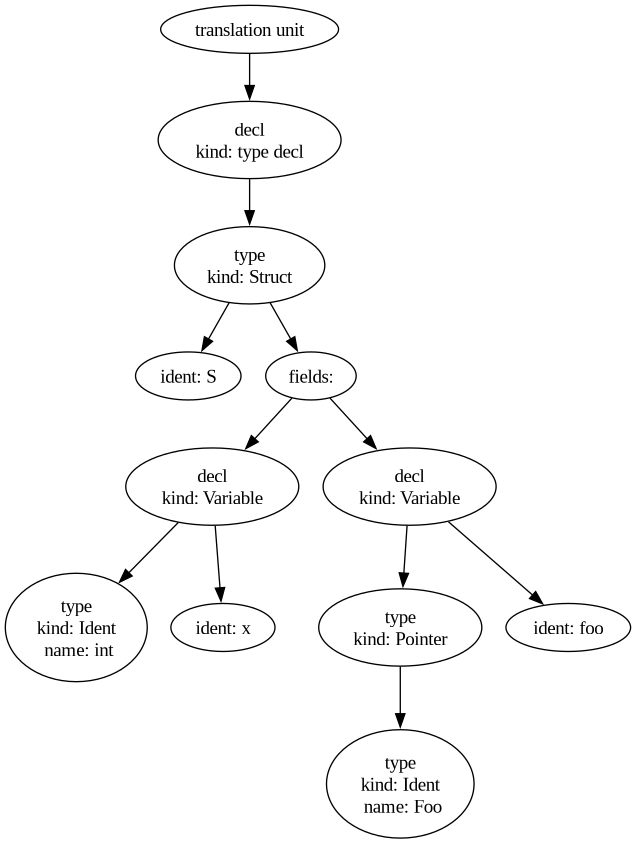
\includegraphics[width=\textwidth,height=0.8\textheight,keepaspectratio]{ex_out.png}
\centering
\end{figure}

\newpage
\paragraph{Аналогично визуализируем определение:}
\label{graphviz:decl}
\beginminteddef{c}
int *(*x())[], y, *z;
\end{minted}

\begin{figure}[H]
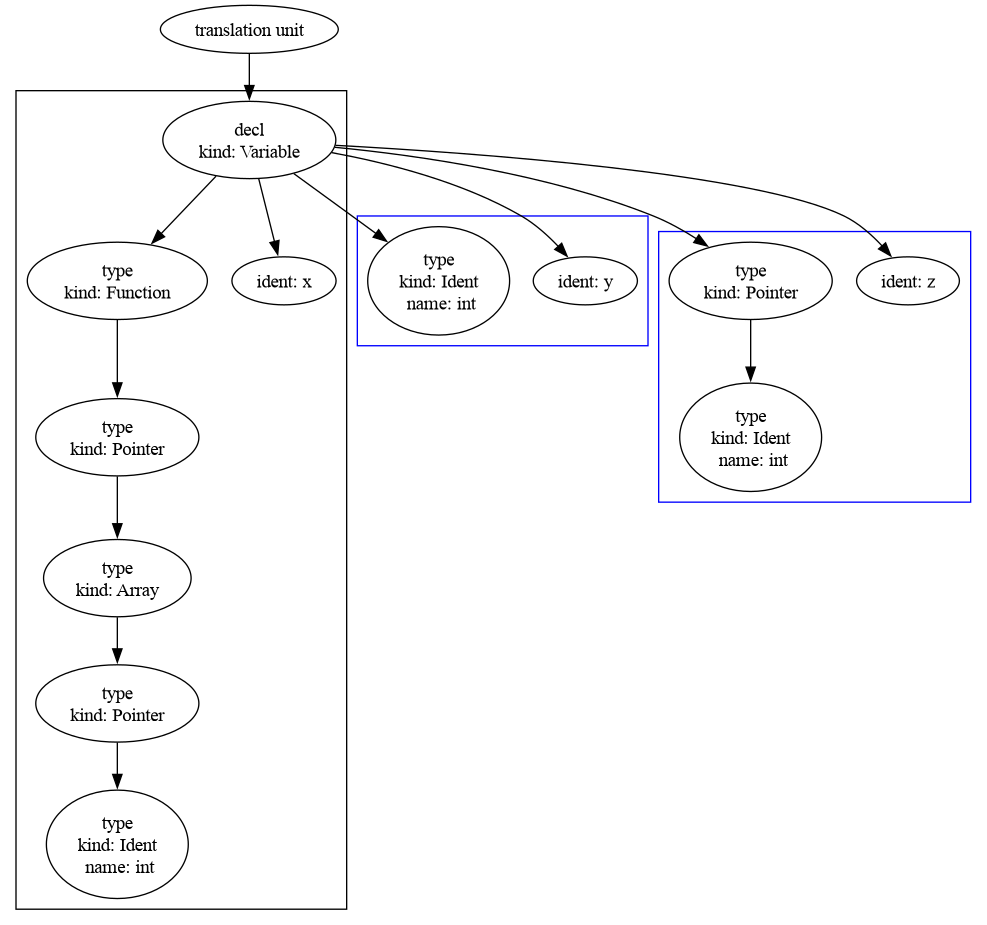
\includegraphics[width=\textwidth,height=\textheight,keepaspectratio]{ty_out.png}
\centering
\end{figure}

\newpage
\paragraph{Аналогично визуализируем выражение:}
\label{graphviz:expr}

\beginminteddef{c}
x = (a = a1) && b == c || d
\end{minted}

\begin{figure}[H]
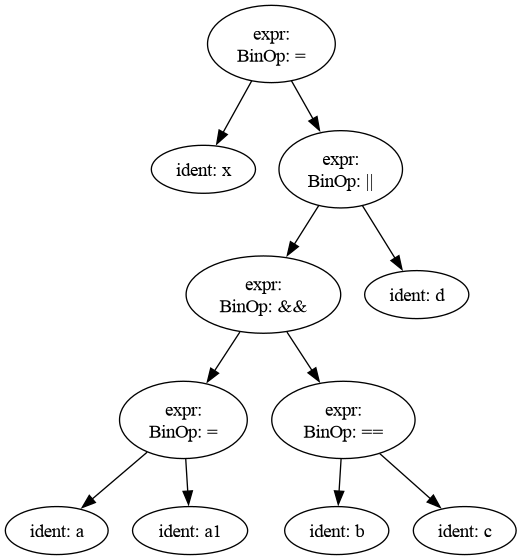
\includegraphics[width=\textwidth,height=\textheight,keepaspectratio]{expr_out.png}
\centering
\end{figure}

% \section {Расширение Си}



% \subsection{@ директивы}

% Была добавлена поддержка \@ деректив, имеющих следующую грамматику:

% at-directive:

% \qquad @ identifier

% \qquad @ identifier(argument-expression-list\textsubscript{opt})


% \subsection{Анализ AST}


\newpage
% \addcontentsline{toc}{section}{Заключение}
\section{Заключение}

Написанная мной библиотека может быть использованна для написания утилит, обрабатывающих код языка программирования Си, 
а также в качестве source-to-source компилятора языка Extended C.


\newpage
\section{Приложения}

\subsection{Проекты}
\paragraph{Проект:} \label{extras:ecc} 
\url{https://github.com/m-blg/c_lang}

\paragraph{Библиотека с основными примитивами:} \label{extras:c-core}
\url{https://github.com/m-blg/c_core}


\subsection{Примитивы}
\subsubsection{Аллокаторы}
\begin{code}
  \inputminted[breaklines=true, xleftmargin=1em, linenos, frame=single,
  framesep=10pt, fontsize=\footnotesize]
  {c}{listings/intro/c_alloc.c}
  \caption{glibc аллокатор}
  \label{extras:glibc_alloc}
\end{code}
\begin{code}
  \inputminted[breaklines=true, xleftmargin=1em, linenos, frame=single,
  framesep=10pt, fontsize=\footnotesize]
  {c}{listings/intro/arena.c}
  \caption{Арена аллокатор}
  \label{extras:arena_alloc}
\end{code}

\subsubsection{Форматтер}
\begin{code}
  \inputminted[breaklines=true, xleftmargin=1em, linenos, frame=single,
  framesep=10pt, fontsize=\footnotesize]
  {c}{listings/intro/fmt.c}
  \caption{Имплементация основных методов StringFormatter}
  \label{extras:fmt_impl}
\end{code}


\subsection{Лексический разбор}

\subsubsection{Определения Си}
\begin{code}
  \inputminted[breaklines=true, xleftmargin=1em, linenos, frame=single,
  framesep=10pt, fontsize=\footnotesize]
  {c}{listings/lexing/def.h}
	\caption{defs.h}
    \label{extras:c_defs}
\end{code}

\subsubsection{Структура токена Си}
\begin{code}
  \inputminted[breaklines=true, xleftmargin=1em, linenos, frame=single,
  framesep=10pt, fontsize=\footnotesize]
  {c}{listings/lexing/token.c}
	\caption{Структура токена Си}
    \label{extras:c_token}
\end{code}

\subsubsection{Примеры функций лексического разбора}
\begin{code}
  \inputminted[breaklines=true, xleftmargin=1em, linenos, frame=single,
  framesep=10pt, fontsize=\footnotesize]
  {c}{listings/lexing/lexer_fns.c}
	\caption{Примеры функций лексического разбора}
    \label{extras:lexer_fns}
\end{code}

\subsubsection{Функции отладочного форматирования токенов}
\begin{code}
  \inputminted[breaklines=true, xleftmargin=1em, linenos, frame=single,
  framesep=10pt, fontsize=\footnotesize]
  {c}{listings/lexing/token.c}
	\caption{Функции отладочного форматирования токенов}
    \label{extras:token_dbg_print}
\end{code}


\subsubsection{Функция препроцессора}
\begin{code}
  \inputminted[breaklines=true, xleftmargin=1em, linenos, frame=single,
  framesep=10pt, fontsize=\footnotesize]
  {c}{listings/pp/tokenize.c}
  \caption{Реализация препроцессора}
  \label{extras:pp}
\end{code}\


\subsection{Грамматический разбор}
\subsubsection{Абстрактное синтаксическое дерево}
\begin{code}
  \inputminted[breaklines=true, xleftmargin=1em, linenos, frame=single,
  framesep=10pt, fontsize=\footnotesize]
  {c}{listings/parsing/ast.c}
  \caption{C AST}
  \label{extras:c_ast}
\end{code}\

\subsubsection{Функции разбора выражений}
\begin{code}
  \inputminted[breaklines=true, xleftmargin=1em, linenos, frame=single,
  framesep=10pt, fontsize=\footnotesize]
  {c}{listings/parsing/expr.c}
  \caption{Функции разбора выражений}
  \label{extras:parse_expr}
\end{code}\

\subsubsection{Функции разбора определений}
\begin{code}
  \inputminted[breaklines=true, xleftmargin=1em, linenos, frame=single,
  framesep=10pt, fontsize=\footnotesize]
  {c}{listings/parsing/decl.c}
  \caption{Функции разбора определений}
  \label{extras:parse_decl}
\end{code}\

\subsubsection{Функции разбора утдверждений}
\begin{code}
  \inputminted[breaklines=true, xleftmargin=1em, linenos, frame=single,
  framesep=10pt, fontsize=\footnotesize]
  {c}{listings/parsing/stmt.c}
  \caption{Функции разбора утдверждений}
  \label{extras:parse_stmt}
\end{code}\

\subsubsection{Функция разбора единицы трансляции}
\begin{code}
  \inputminted[breaklines=true, xleftmargin=1em, linenos, frame=single,
  framesep=10pt, fontsize=\footnotesize]
  {c}{listings/parsing/tr_unit.c}
  \caption{Функция разбора единицы трансляции}
  \label{extras:parse_tr_unit}
\end{code}\


\subsection{Трансляция Ast}
\subsubsection{Пример функций трансляции AST обратно в Си}
\begin{code}
  \inputminted[breaklines=true, xleftmargin=1em, linenos, frame=single,
  framesep=10pt, fontsize=\footnotesize]
  {c}{listings/translation/unparse/unparse.c}
  \caption{Функции трансляции AST в Си}
  \label{extras:unparse}
\end{code}\

\subsubsection{Пример функций трансляции AST в graphviz}
% label always after caption
\begin{code}
  \inputminted[breaklines=true, xleftmargin=1em, linenos, frame=single,
  framesep=10pt, fontsize=\footnotesize]
  {c}{listings/translation/ast_vis/graphviz.c}
  \caption{Функции трансляции в graphviz}
  \label{extras:compile-graphviz}
\end{code}\